\documentclass[12pt]{article}
\usepackage{color,latexsym,fancyhdr,amsmath,amsfonts,dsfont,amssymb,graphicx}
\usepackage{color,soul}
%\graphicspath{{}}


\topmargin        -0.2 in
\textheight       8.4 in
\oddsidemargin    0 in  
\evensidemargin   0 in     
\textwidth        6.5 in
\headheight       15pt     
\headsep          .35 in     


\begin{document}
\pagestyle{fancy} \lhead{CS 421 Homework} \chead{\textcolor{red}{02/22/2019}}
\rhead{\textcolor{red}{Austin Klum}} 
\lfoot{} \cfoot{} \rfoot{}

\begin{enumerate}
	\item[1]
	\item[]
		x := x * b + 3\\
		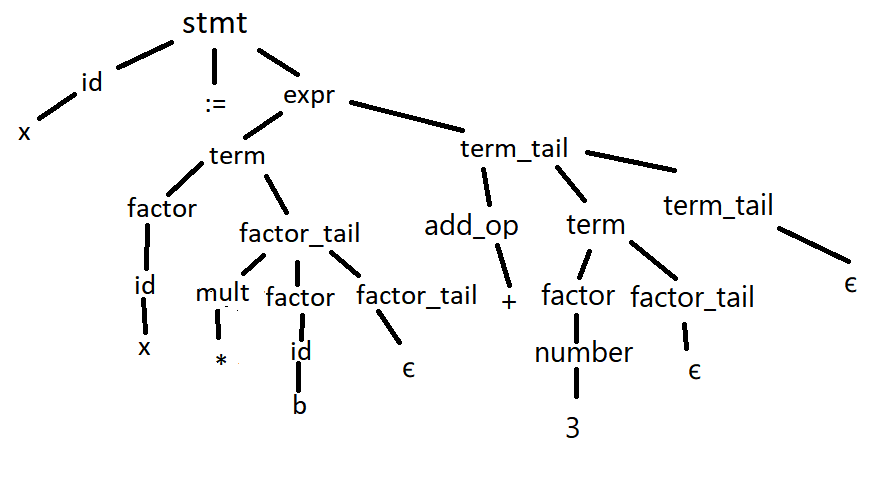
\includegraphics[scale=.5]{hw01-1a.png}\\
		a := b / c * d\\
		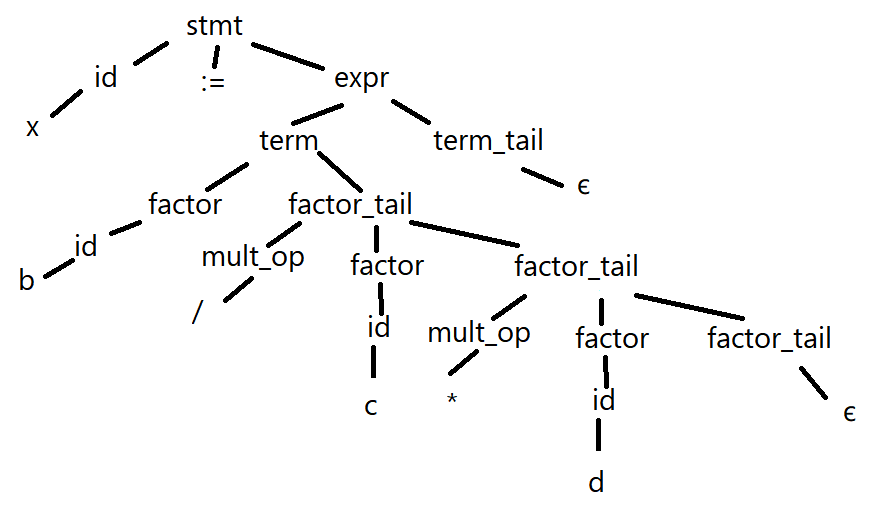
\includegraphics[scale=.5]{hw01-1b.png}\\
		j := k + i * j - 7\\
		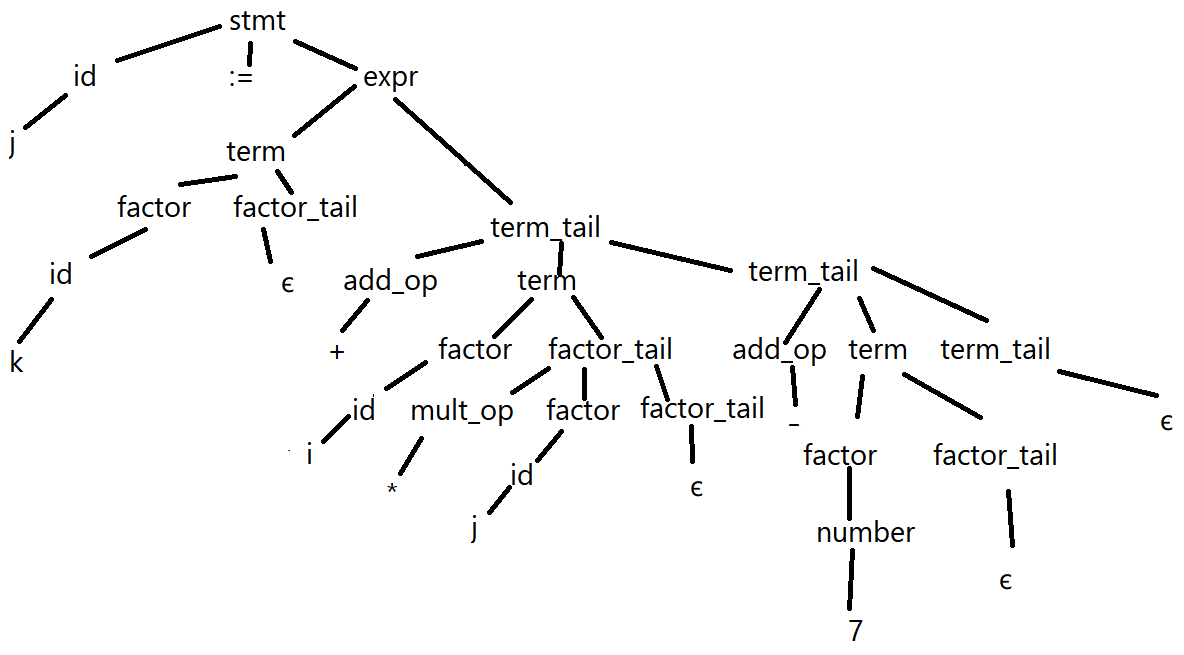
\includegraphics[scale=.5]{hw01-1c.png}\\
	\item[2]
		\begin{enumerate}
			\item[(a)]\textbf{hoheyheyho}\\
				\begin{align*}
					S &\Rightarrow \text{Y}\\
					  &\Rightarrow \text{ho S hey Z} \\
					  &\Rightarrow \text{ho S heyheyho} \\
					  &\Rightarrow \text{ho Z heyheyho} \\
					  &\Rightarrow \text{ho $ \epsilon $ heyheyho} \\
					  &\Rightarrow \text{hoheyheyho} \\
				\end{align*}
			\item[(b)] The grammar is ambiguous as there are multiple ways to derive the same sequence. For example \textbf{hohey} can be derived by
				\begin{align*}
					S &\Rightarrow \text{Y}\\
					&\Rightarrow \text{ho S hey S} \\
					&\Rightarrow \text{ho S hey Z} \\
					&\Rightarrow \text{ho S hey $ \epsilon $} \\
					&\Rightarrow \text{ho Z hey} \\
					&\Rightarrow \text{ho $ \epsilon $ hey} \\
					&\Rightarrow \text{hohey} \\
				\end{align*}
			Or it can be derived by
				\begin{align*}
					S &\Rightarrow \text{Z}\\
					  &\Rightarrow \text{hohey}
				\end{align*}
		\end{enumerate}		
	\item[3]
		\begin{enumerate}
			\item[(a)]
				\begin{align*}
					S &\rightarrow xA \\
					  &\rightarrow yA \\
					  &\rightarrow \_A \\
					A &\rightarrow xB \\
					  &\rightarrow yB \\
					  &\rightarrow \_B \\
					  &\rightarrow 0B \\
					  &\rightarrow 1B \\
					  &\rightarrow \epsilon \\
					B &\rightarrow xA \\
				      &\rightarrow yA \\
				      &\rightarrow \_A \\
				      &\rightarrow 0A \\
					  &\rightarrow 1A \\
					  &\rightarrow \epsilon \\
				\end{align*}
			\item[(b)]
				\begin{align*}
					S &\Rightarrow xA \\
					  &\Rightarrow xyB \\
					  &\Rightarrow xyxA \\
					  &\Rightarrow xyx\_B \\
					  &\Rightarrow xyx\_0A \\
					  &\Rightarrow xyx\_01B \\
					  &\Rightarrow xyx\_011A \\
					  &\Rightarrow xyx\_011\epsilon \\
					  &\Rightarrow xyx\_011 \\
				\end{align*}
		\end{enumerate}
	\item[4]
		\begin{align*}
			S &\rightarrow aaAa \\
			A &\rightarrow aaAa \\
			  &\rightarrow B \\
			B &\rightarrow bB \\
		      &\rightarrow \epsilon
		\end{align*}
		We know this will generate only the strings we are looking for as we ensure that once we reach the B state we can no longer add to the a characters. This allows us to make sure we maintain the proper amount of a's and allowing for as many b's as needed.
	\item[5]
		\begin{align*}
			S &\rightarrow aCb\\
			  &\rightarrow aA\\
			A &\rightarrow aA\\
			  &\rightarrow \epsilon\\
			B &\rightarrow bB\\
			  &\rightarrow \epsilon\\
			C &\rightarrow aCb\\
			  &\rightarrow aA\\
			  &\rightarrow abbB\\
		\end{align*}
		We know this will generate only the strings we are looking for as we ensure that, by adding our state C, we can never hit the condition of the a's and b's begin equal.
\end{enumerate}
 
\end{document}


